\documentclass[11pt]{article}
\usepackage[utf8]{inputenc}
\usepackage[brazilian]{babel}

\usepackage{subfigure}
\usepackage{indentfirst}
\usepackage{graphicx}
\usepackage{xcolor}
\usepackage[cm]{fullpage}
\usepackage{hyperref}

\usepackage{enumitem}

\graphicspath{ {images/} }

\newlist{legal}{enumerate}{10}
\setlist[legal]{label*=\arabic*.}

\usepackage{listings}
\lstset{
  basicstyle=\footnotesize\ttfamily,
}

\newcommand*{\alert}[1]{\vspace{0.4cm}\colorbox{gray!60!white}{\parbox{0.92\linewidth}{{\centering \textbf{IMPORTANTE!}\\}#1}}\vspace{0.4cm}}

\title{Guia Básico do Github Classroom:\\Criação de Grupos e Envio dos Trabalhos Práticos}

\author{Fernando Jorge Mota e Márcio Castro\\[0.3em]
\small Universidade Federal de Santa Catarina}
\date{}

\hyphenation{tool-chain}

\usepackage{url}

\begin{document}

\maketitle

\section{Introdução}

Nesse semestre, será usado uma ferramenta chamada \textit{Github Classroom} para o envio das tarefas e trabalhos. Diferente do \textit{Moodle}, essa ferramenta não permite o envio de arquivos compactados, mas sim um repositório gerenciado pelo \textit{Git}. Por isso, é importante saber usar o \textit{Git} de forma a poder armazenar o desenvolvimento do projeto e também saber usar o \textit{Github Classroom} para a criação e participação dos grupos nas atividades.

\section{Git}

O \textit{Git} é um sistema de controle de versões distribuído, criado por Linus Torvalds para uso no desenvolvimento do \textit{kernel} do Linux e que tem como principal característica permitir o trabalho de uma \textbf{equipe} de forma colaborativa, como por exemplo possível criar diferentes bifurcações (\textit{branches}) do projeto com o objetivo de testar diferentes possibilidades e então, no final, juntar tudo em uma versão final do trabalho.

Existem três principais formas de utilização do \textit{Git}:

\begin{enumerate}
\item Usar a ferramenta \texttt{git}\footnote{A ferramenta pode ser instalada no Ubuntu utilizando-se o seguinte comando: \texttt{sudo apt-get install git}} no terminal (disponível para Linux, MacOS e Windows);
\item Usar uma ferramenta gráfica, que permite visualizar e gerenciar o estado do repositório de maneira visual, como o \textit{SmartGit}\footnote{Disponível em: \url{https://www.syntevo.com/smartgit/}} e o \textit{Github Desktop}\footnote{Disponível em: \url{https://desktop.github.com}};
\item Usar a própria interface \textit{web} que o \textit{Github} disponibiliza para envio das modificações.
\end{enumerate}

Observe que não é necessário um domínio técnico completo do \textit{Git} para a realização das atividades da disciplina. Entretanto, mesmo seu domínio básico já deve auxiliar na resolução de alguns problemas, como o compartilhamento do código entre os membros do grupo, a resolução de dúvidas com o monitor ou o professor, e também o teste de diferentes alternativas para resolução do problema. Por domínio básico, entende-se:

\begin{itemize}
  \item Saber como replicar todo o repositório (\texttt{git clone});
  \item Saber como baixar atualizações do repositório (\texttt{git pull});
  \item Saber como registrar alterações no repositório (\texttt{git add} e \texttt{git commit});
  \item Saber como enviar as alterações para o repositório (\texttt{git push}); e
  \item Saber como resolver conflitos que porventura possam acontecer devido ao uso do repositório por mais de um membro do grupo.
\end{itemize}

Mais informações sobre a ferramenta \texttt{git} podem ser encontradas nos links abaixo:

\begin{itemize}
\item \url{https://try.github.com}: Ferramenta interativa desenvolvida pelo próprio \textit{Github} para aprendizado das funcionalidades básicas do \textit{Git}. \textbf{Extremamente recomendado} para quem nunca usou o \textit{Git} e quer ter domínio básico da ferramenta;
\item \url{https://guides.github.com/}: Guias desenvolvidos pelo \textit{Github} para uso do \textit{Git} e do próprio serviço;
\item \url{https://git-scm.com/about}: Livro gratuito e completo sobre o \textit{Git};
\item \url{https://www.syntevo.com/smartgit/}: Cliente \textit{Git} completo com interface gráfica e suporte para Linux, Mac e Windows. Gratuito para uso não-comercial; e
\item \url{https://desktop.github.com/}: Cliente \textit{Git} desenvolvido pelo \textit{Github} com o propósito de ser mais simples, amigável e fornecer melhor integração com o \textit{Github}. Totalmente gratuito e disponível para Windows e MacOS.
\end{itemize}

\section{Github Classroom}

O \textit{Github Classroom} é uma ferramenta desenvolvida pelo \textit{Github} que permite o envio de tarefas e trabalhos através da criação de repositórios \textit{Git} para cada grupo e/ou estudante. Para o estudante, seu uso é bem simples: basta entrar no \textit{link} disponibilizado pelo professor, criar um grupo (ou entrar em algum grupo já existente) e então usar o repositório criado pela ferramenta para o grupo em questão para gerenciamento do código do trabalho.

\alert{Não há, para o \textit{Github Classroom}, uma etapa específica para ``envio do código'': o professor irá recuperar a solução proposta pelos alunos na \textit{branch} \textit{master} do repositório (considerada principal pelo \textit{Git}). \textbf{Para o \textit{Github Classroom}, é oficializado como envio o último \textit{commit} disponível na \textit{branch} \textit{master} do repositório do grupo na data e hora de entrega do trabalho especificadas pelo professor da disciplina para o trabalho ou atividade em questão.}}

Note que serão disponibilizados para avaliação todas as informações armazenadas no repositório. Isso inclui lista de pessoas que enviaram \textit{commits} para o repositório, assim como mensagens de \textit{commit}, data e hora de cada \textit{commit} e também as alterações feitas no projeto, além de outras informações. Entretanto, será avaliado efetivamente apenas a versão final do trabalho, conforme o estado do último \textit{commit} realizado antes da data e hora de entrega do trabalho.

Por isso, é recomendado o registro (\textit{commit}) e subsequente envio (\textit{push}) do envio do trabalho para o \textit{Github} conforme a solução vai sendo desenvolvida, uma vez que isso possibilita compartilhamento do código com os colegas e com outros dispositivos do próprio estudante, além de garantir uma cópia de segurança caso aconteça algum problema com o computador onde estava sendo desenvolvida a solução.

\subsection{Instruções para criação de um novo grupo (ou participação em um grupo) no \textit{Github Classroom}}

Para criação de um novo grupo (ou participação em um grupo existente) no \textit{Github Classroom}, é necessário que o aluno tenha:

\begin{itemize}
  \item Entrado em um dos grupos pré-definidos no \textit{Moodle} da disciplina para o trabalho em questão; e
  \item Criado uma conta gratuita no \textit{Github} (\url{https://github.com}).
\end{itemize}

Depois, basta seguir os seguintes passos para poder criar ou entrar em um grupo no \textit{Github Classroom}:

\begin{enumerate}
  \item Entrar no \textit{link} disponibilizado pelo professor para a atividade\footnote{O \textit{link} a ser disponibilizado pelo professor terá o seguinte formato: \url{https://classroom.github.com/g/<hash_aleatorio>}};
  \item Escolher \textbf{o seu} número de matrícula conforme imagem do \textit{site} mostrada abaixo. Este procedimento deverá ser feito uma única vez ao acessar o \textit{Github Classroom} em alguma atividade da disciplina e será usado pelo professor para associação com os dados presentes no \textit{Moodle}. 

  \begin{center}
    \vspace{0.2cm}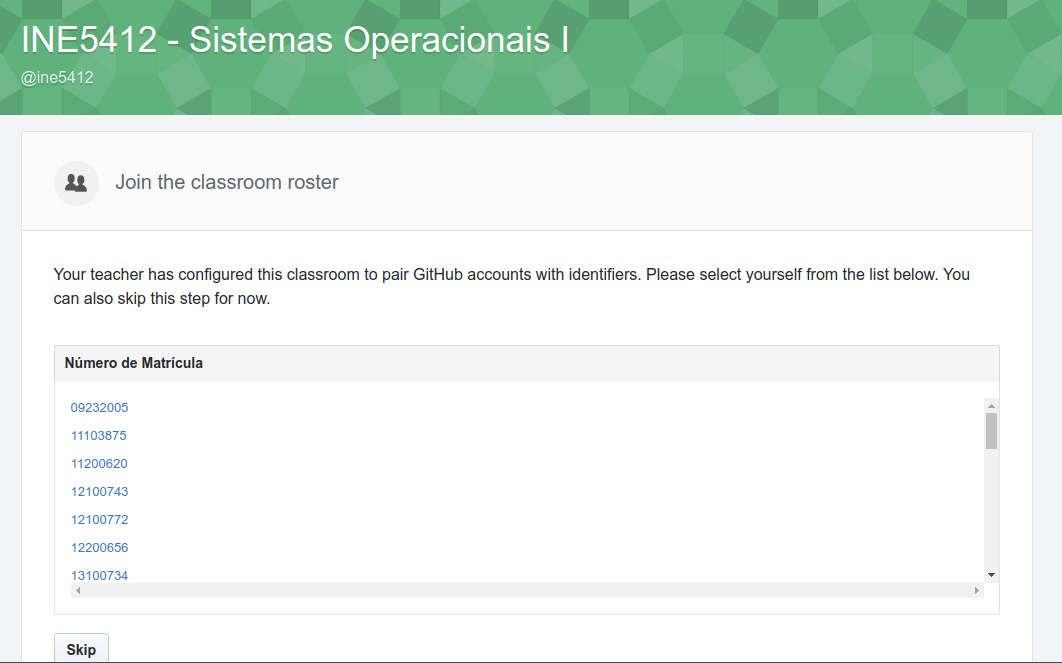
\includegraphics[width=0.8\textwidth]{roaster}
  \end{center}

  \item Depois de selecionar seu número de matricula, será disponibilizado a lista de grupos já criados para aquela tarefa pelo seus colegas e será disponibilizado a opção para criar um grupo, como mostrado abaixo.

  \begin{center}
  \vspace{0.2cm}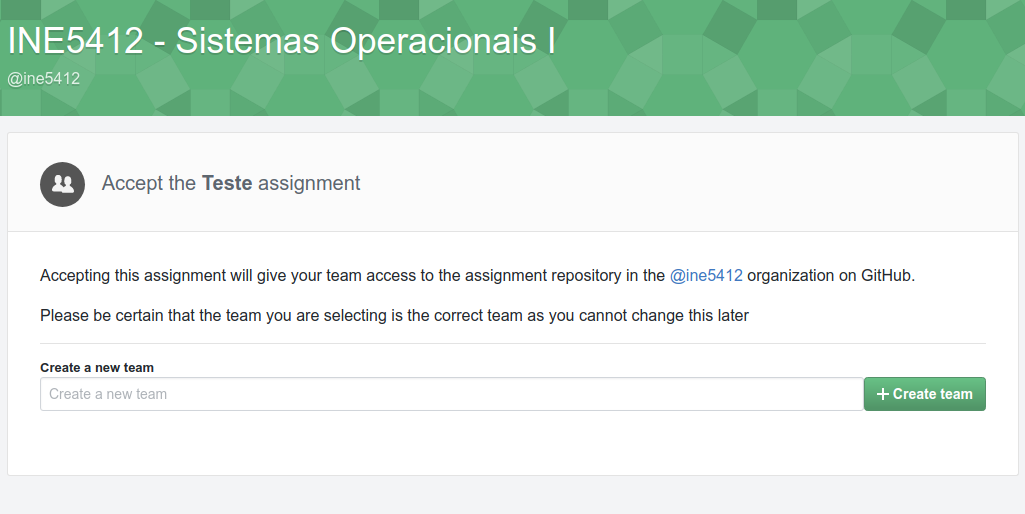
\includegraphics[width=0.8\textwidth]{create-group}
  \end{center}

  \newpage
  
  \item Após criar ou entrar em um grupo, o \textit{Github Classroom} disponibilizará o \textit{link} para o repositório \textit{Git} do seu grupo, conforme mostrado abaixo.

  \begin{center}
    \vspace{0.2cm}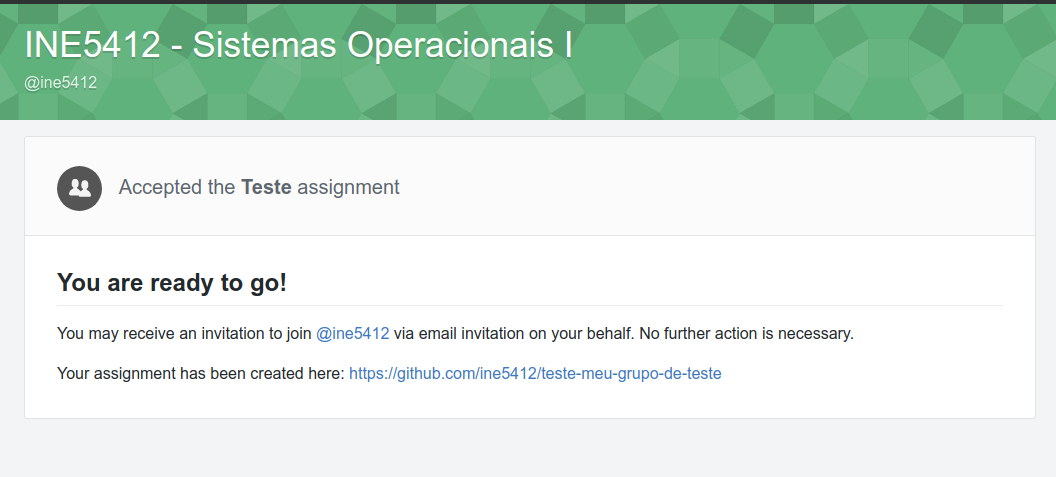
\includegraphics[width=0.8\textwidth]{repository-created}
  \end{center}
  
  \item Observe que, nos primeiros momentos após o repositório ser criado, será exibida tela abaixo avisando que o \textit{Github} está copiando o código base do \textbf{Nanvix} (Sistema Operacional usado pela disciplina) para o seu repositório. Em seguida, basta fazer a clonagem do repositório para o seu computador e começar a trabalhar.

  \begin{center}
    \vspace{0.2cm}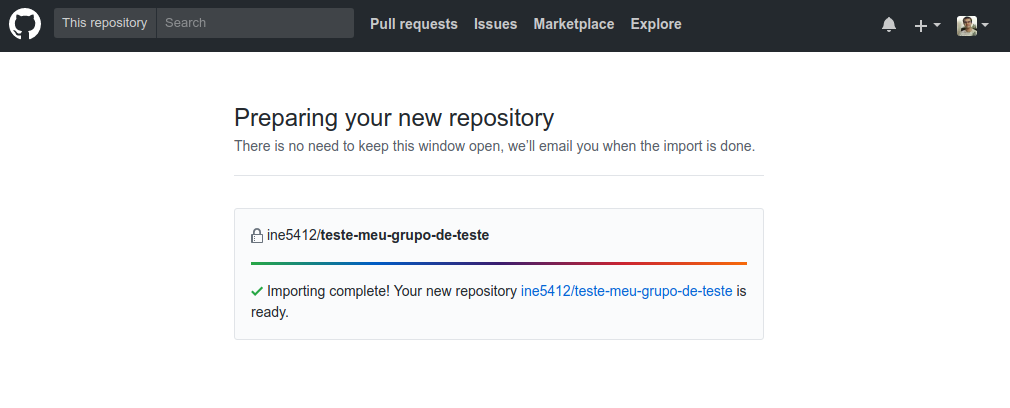
\includegraphics[width=0.8\textwidth]{repository-forked}
  \end{center}

%  \alert{Embora o \textit{Github} também copie \textit{branches} como \textit{dev}, \textit{security} e \textit{master-intlvl-hotfix}, a \textbf{\textit{branch} que deverá ser usada nos trabalhos e atividades da disciplina} é a \textit{branch \textbf{master}}. Entretanto, é permitido ao aluno criar novas \textit{branches} com base na \textit{branch master}, desde que todo o resultado final do trabalho seja disponibilizado na própria \textit{branch master}.}
\end{enumerate}
\end{document}
